\documentclass{ctexbeamer}
\usepackage{amsmath,amssymb}
\usepackage{amsthm}
\usepackage{subfig}
\usepackage{graphicx}
\usepackage[defaultmono,scale=0.85]{droidsansmono}
% \usepackage{tikz}
\usepackage{minted}
\usepackage{color}
% \usepackage{mdframed}
% \usepackage[colorlink=true,xetex]{hyperref}

\usetheme{Madrid}
\usefonttheme[onlymath]{serif}
\definecolor{codebg}{rgb}{0.95,0.95,0.95}
% \surroundwithmdframed{minted}

\newcommand{\theauthor}{Sparky\_14145}
\newcommand{\thestudentID}{71XXXXXX}
\newcommand{\theemail}{me@example.com}
\newcommand{\theinst}{College of Software Engineering}
\newcommand{\theshortinst}{CoSE}

\input{personal_info/info.tex}

\author{
    \thestudentID
    \theauthor
    \thanks{Email: \theemail}
}
\institute[\theshortinst]{\theinst}
\title{B\'ezier 曲线}
\subtitle{计算机图形学 作业四}

\begin{document}
    \begin{frame}
        \titlepage
    \end{frame}

    \begin{frame}
        \frametitle{目录}
        \tableofcontents
    \end{frame}

    \section{B\'ezier 曲线绘制}

    \begin{frame}[fragile]
        \frametitle{B\'ezier 曲线绘制}
    
        按照作业文档中的说明来实现。 \pause
        {
            \small
            \begin{minted}[linenos,autogobble,bgcolor=codebg,breaklines]{cpp}
void bezier(const std::vector<cv::Point2f> &control_points, cv::Mat &window) {
    const float delta_t = 0.001; // [1]
    for (float t = 0; t <= 1; t += delta_t) {
        cv::Point point = recursive_bezier(control_points, t);
        window.at<cv::Vec3b>(point.y, point.x)[1] = 255; // [2]
    }

}
            \end{minted}
        }

        取一个较小的 $\Delta t$(如 \verb|[1]| 所示),然后从 0 开始,每次将 $t$ 加上
        $\Delta t$,找到 de Casteljau 算法确定出的那个点,绘制出来。\pause

        为了方便区分,我将这种实现绘制的点表示成绿色(如 \verb|[2]| 所示)。
    \end{frame}

    \section{de Casteljau 算法}
    \begin{frame}[fragile]
        \frametitle{de Casteljau 算法}
    
        代码如下:

        {
            \small
            \begin{minted}[autogobble,linenos,bgcolor=codebg,breaklines]{cpp}
cv::Point2f recursive_bezier(const std::vector<cv::Point2f> &control_points, float t) {
    std::vector<cv::Point2f> res = control_points, tmp;
    while (res.size() > 1) {
        for (size_t i = 1; i < res.size(); ++i) {
            tmp.push_back(t * res[i] + (1-t) * res[i-1]);
        }
        res.swap(tmp);
        tmp.clear();
    }
    return res[0];
}
            \end{minted}
        }
    
    \end{frame}

    \begin{frame}[fragile]

        {
            \small
            \begin{minted}[autogobble,linenos,bgcolor=codebg,breaklines,highlightlines={2}]{cpp}
cv::Point2f recursive_bezier(const std::vector<cv::Point2f> &control_points, float t) {
    std::vector<cv::Point2f> res = control_points, tmp;
    while (res.size() > 1) {
        for (size_t i = 1; i < res.size(); ++i) {
            tmp.push_back(t * res[i] + (1-t) * res[i-1]);
        }
        res.swap(tmp);
        tmp.clear();
    }
    return res[0];
}
            \end{minted}
        }

        \parbox[c][0.2\textheight][c]{\textwidth}{
            创建两个 \texttt{vector},其中 \texttt{res} 保存上一轮迭代计算出的点集;
            而 \texttt{tmp} 用来保存当前轮次迭代中计算出的结果。
        }

    \end{frame}

    \begin{frame}[fragile]

        {
            \small
            \begin{minted}[autogobble,linenos,bgcolor=codebg,breaklines,highlightlines={3,9}]{cpp}
cv::Point2f recursive_bezier(const std::vector<cv::Point2f> &control_points, float t) {
    std::vector<cv::Point2f> res = control_points, tmp;
    while (res.size() > 1) {
        for (size_t i = 1; i < res.size(); ++i) {
            tmp.push_back(t * res[i] + (1-t) * res[i-1]);
        }
        res.swap(tmp);
        tmp.clear();
    }
    return res[0];
}
            \end{minted}
        }

        \parbox[c][0.2\textheight][c]{\textwidth}{
            按照算法,我们需要不断重复计算,直到结果点集中只剩下一个点。
        }

    \end{frame}

    \begin{frame}[fragile]

        {
            \small
            \begin{minted}[autogobble,linenos,bgcolor=codebg,breaklines,highlightlines={4,6}]{cpp}
cv::Point2f recursive_bezier(const std::vector<cv::Point2f> &control_points, float t) {
    std::vector<cv::Point2f> res = control_points, tmp;
    while (res.size() > 1) {
        for (size_t i = 1; i < res.size(); ++i) {
            tmp.push_back(t * res[i] + (1-t) * res[i-1]);
        }
        res.swap(tmp);
        tmp.clear();
    }
    return res[0];
}
            \end{minted}
        }

        \parbox[c][0.2\textheight][c]{\textwidth}{
            第 $k$ 轮迭代共有 $n-k+1$ 个点,于是我们进行 $n-k$ 次计算,每次用相邻的
            2 个点 $P^{(k)}_{i-1}$ 与 $P^{(k)}_i$ 算出下一轮中需要用到的点 $P^{(k+1)}_{i-1}$。
        }

    \end{frame}

    \begin{frame}[fragile]

        {
            \small
            \begin{minted}[autogobble,linenos,bgcolor=codebg,breaklines,highlightlines={5}]{cpp}
cv::Point2f recursive_bezier(const std::vector<cv::Point2f> &control_points, float t) {
    std::vector<cv::Point2f> res = control_points, tmp;
    while (res.size() > 1) {
        for (size_t i = 1; i < res.size(); ++i) {
            tmp.push_back(t * res[i] + (1-t) * res[i-1]);
        }
        res.swap(tmp);
        tmp.clear();
    }
    return res[0];
}
            \end{minted}
        }

        \parbox[c][0.2\textheight][c]{\textwidth}{
            $\overrightarrow{P^{(k)}_{i-1}P^{(k+1)}_{i-1}} = t\cdot\overrightarrow{P^{(k)}_{i-1}P^{(k)}_i}$,
            由此可得 $\overrightarrow{OP^{(k+1)}_{i-1}} = (1-t)\cdot\overrightarrow{OP^{(k)}_{i-1}} + t\cdot\overrightarrow{OP^{(k)}_i}$
        }

    \end{frame}

    \begin{frame}[fragile]

        {
            \small
            \begin{minted}[autogobble,linenos,bgcolor=codebg,breaklines,highlightlines={7,8}]{cpp}
cv::Point2f recursive_bezier(const std::vector<cv::Point2f> &control_points, float t) {
    std::vector<cv::Point2f> res = control_points, tmp;
    while (res.size() > 1) {
        for (size_t i = 1; i < res.size(); ++i) {
            tmp.push_back(t * res[i] + (1-t) * res[i-1]);
        }
        res.swap(tmp);
        tmp.clear();
    }
    return res[0];
}
            \end{minted}
        }

        \parbox[c][0.2\textheight][c]{\textwidth}{
            本轮迭代计算已经完成,将计算结果放入 \texttt{res} 中,并清空缓存 \texttt{tmp}。
        }

    \end{frame}

    \begin{frame}[fragile]

        {
            \small
            \begin{minted}[autogobble,linenos,bgcolor=codebg,breaklines,highlightlines={10}]{cpp}
cv::Point2f recursive_bezier(const std::vector<cv::Point2f> &control_points, float t) {
    std::vector<cv::Point2f> res = control_points, tmp;
    while (res.size() > 1) {
        for (size_t i = 1; i < res.size(); ++i) {
            tmp.push_back(t * res[i] + (1-t) * res[i-1]);
        }
        res.swap(tmp);
        tmp.clear();
    }
    return res[0];
}
            \end{minted}
        }

        \parbox[c][0.2\textheight][c]{\textwidth}{
            结果点集中只剩下了一个点,直接作为结果返回即可。
        }
    \end{frame}

    \section{运行结果}
    \begin{frame}
        \frametitle{运行结果}
    
        这种实现的运行结果如图 \ref{fig:res-1} 所示:

        \begin{figure}
            \centering
            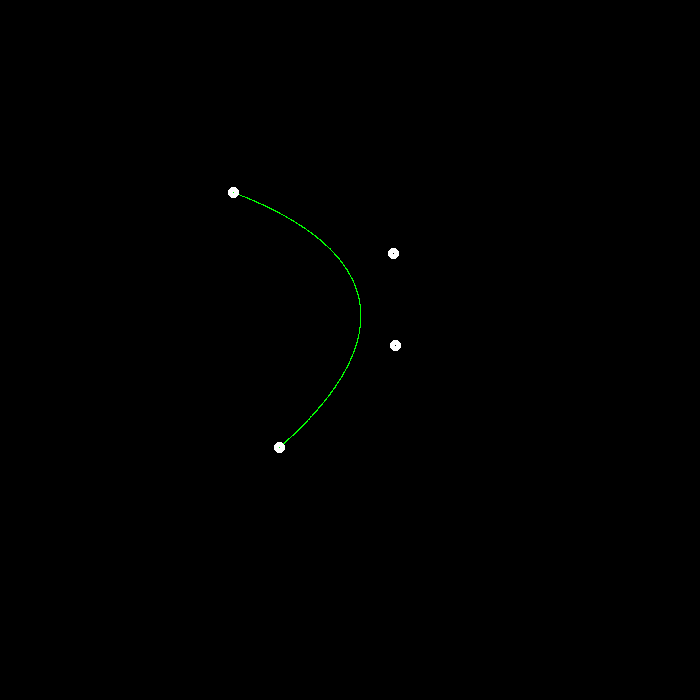
\includegraphics[height=0.6\textheight]{pics/bezier_curve_1.png}
            \caption{第一种实现的运行结果}
            \label{fig:res-1}
        \end{figure}
    
    \end{frame}

    \begin{frame}
        
        而它与教师提供的参考代码共同运行结果如图 \ref{fig:res-2} 所示:

        \begin{figure}
            \centering
            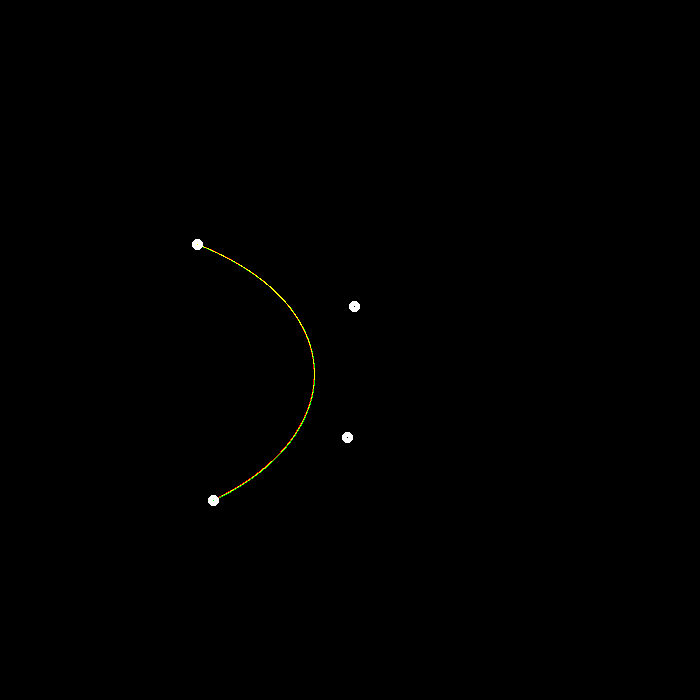
\includegraphics[height=0.6\textheight]{pics/bezier_curve_2.png}
            \caption{两种实现的共同运行结果}
            \label{fig:res-2}
        \end{figure}

        注意其中:教师提供的参考代码绘制出红色曲线,因此两者的重合部分为黄色曲线。

    \end{frame}

    \section{另一种实现}

\end{document}